\section{Monitor electricity consumption}
\SectionPage

\begin{frame}
    \frametitle{Goals}
    \vspace*{\fill}
    Track the energy usage of a large campus, the \ac{BHC}, in Jette, using existing data collected over several years.
    We focus on the academic hospital, that has its own distribution network, in closed-ring shape for increased reliability.

    \textbf{General goals}:
    \begin{itemize}
        \item Having a global view on the data, centralized and well accessible for multiple user
        \item Minimizing the energy losses and overall consumption
        \item Identify where the exact sources of energy cost are
        \item Improve sustainability reducing energy need and peek request
    \end{itemize}

    \vspace*{\fill}
\end{frame}

\begin{frame}
    \frametitle{Context}
    \begin{figure}[ht]
        \fbox{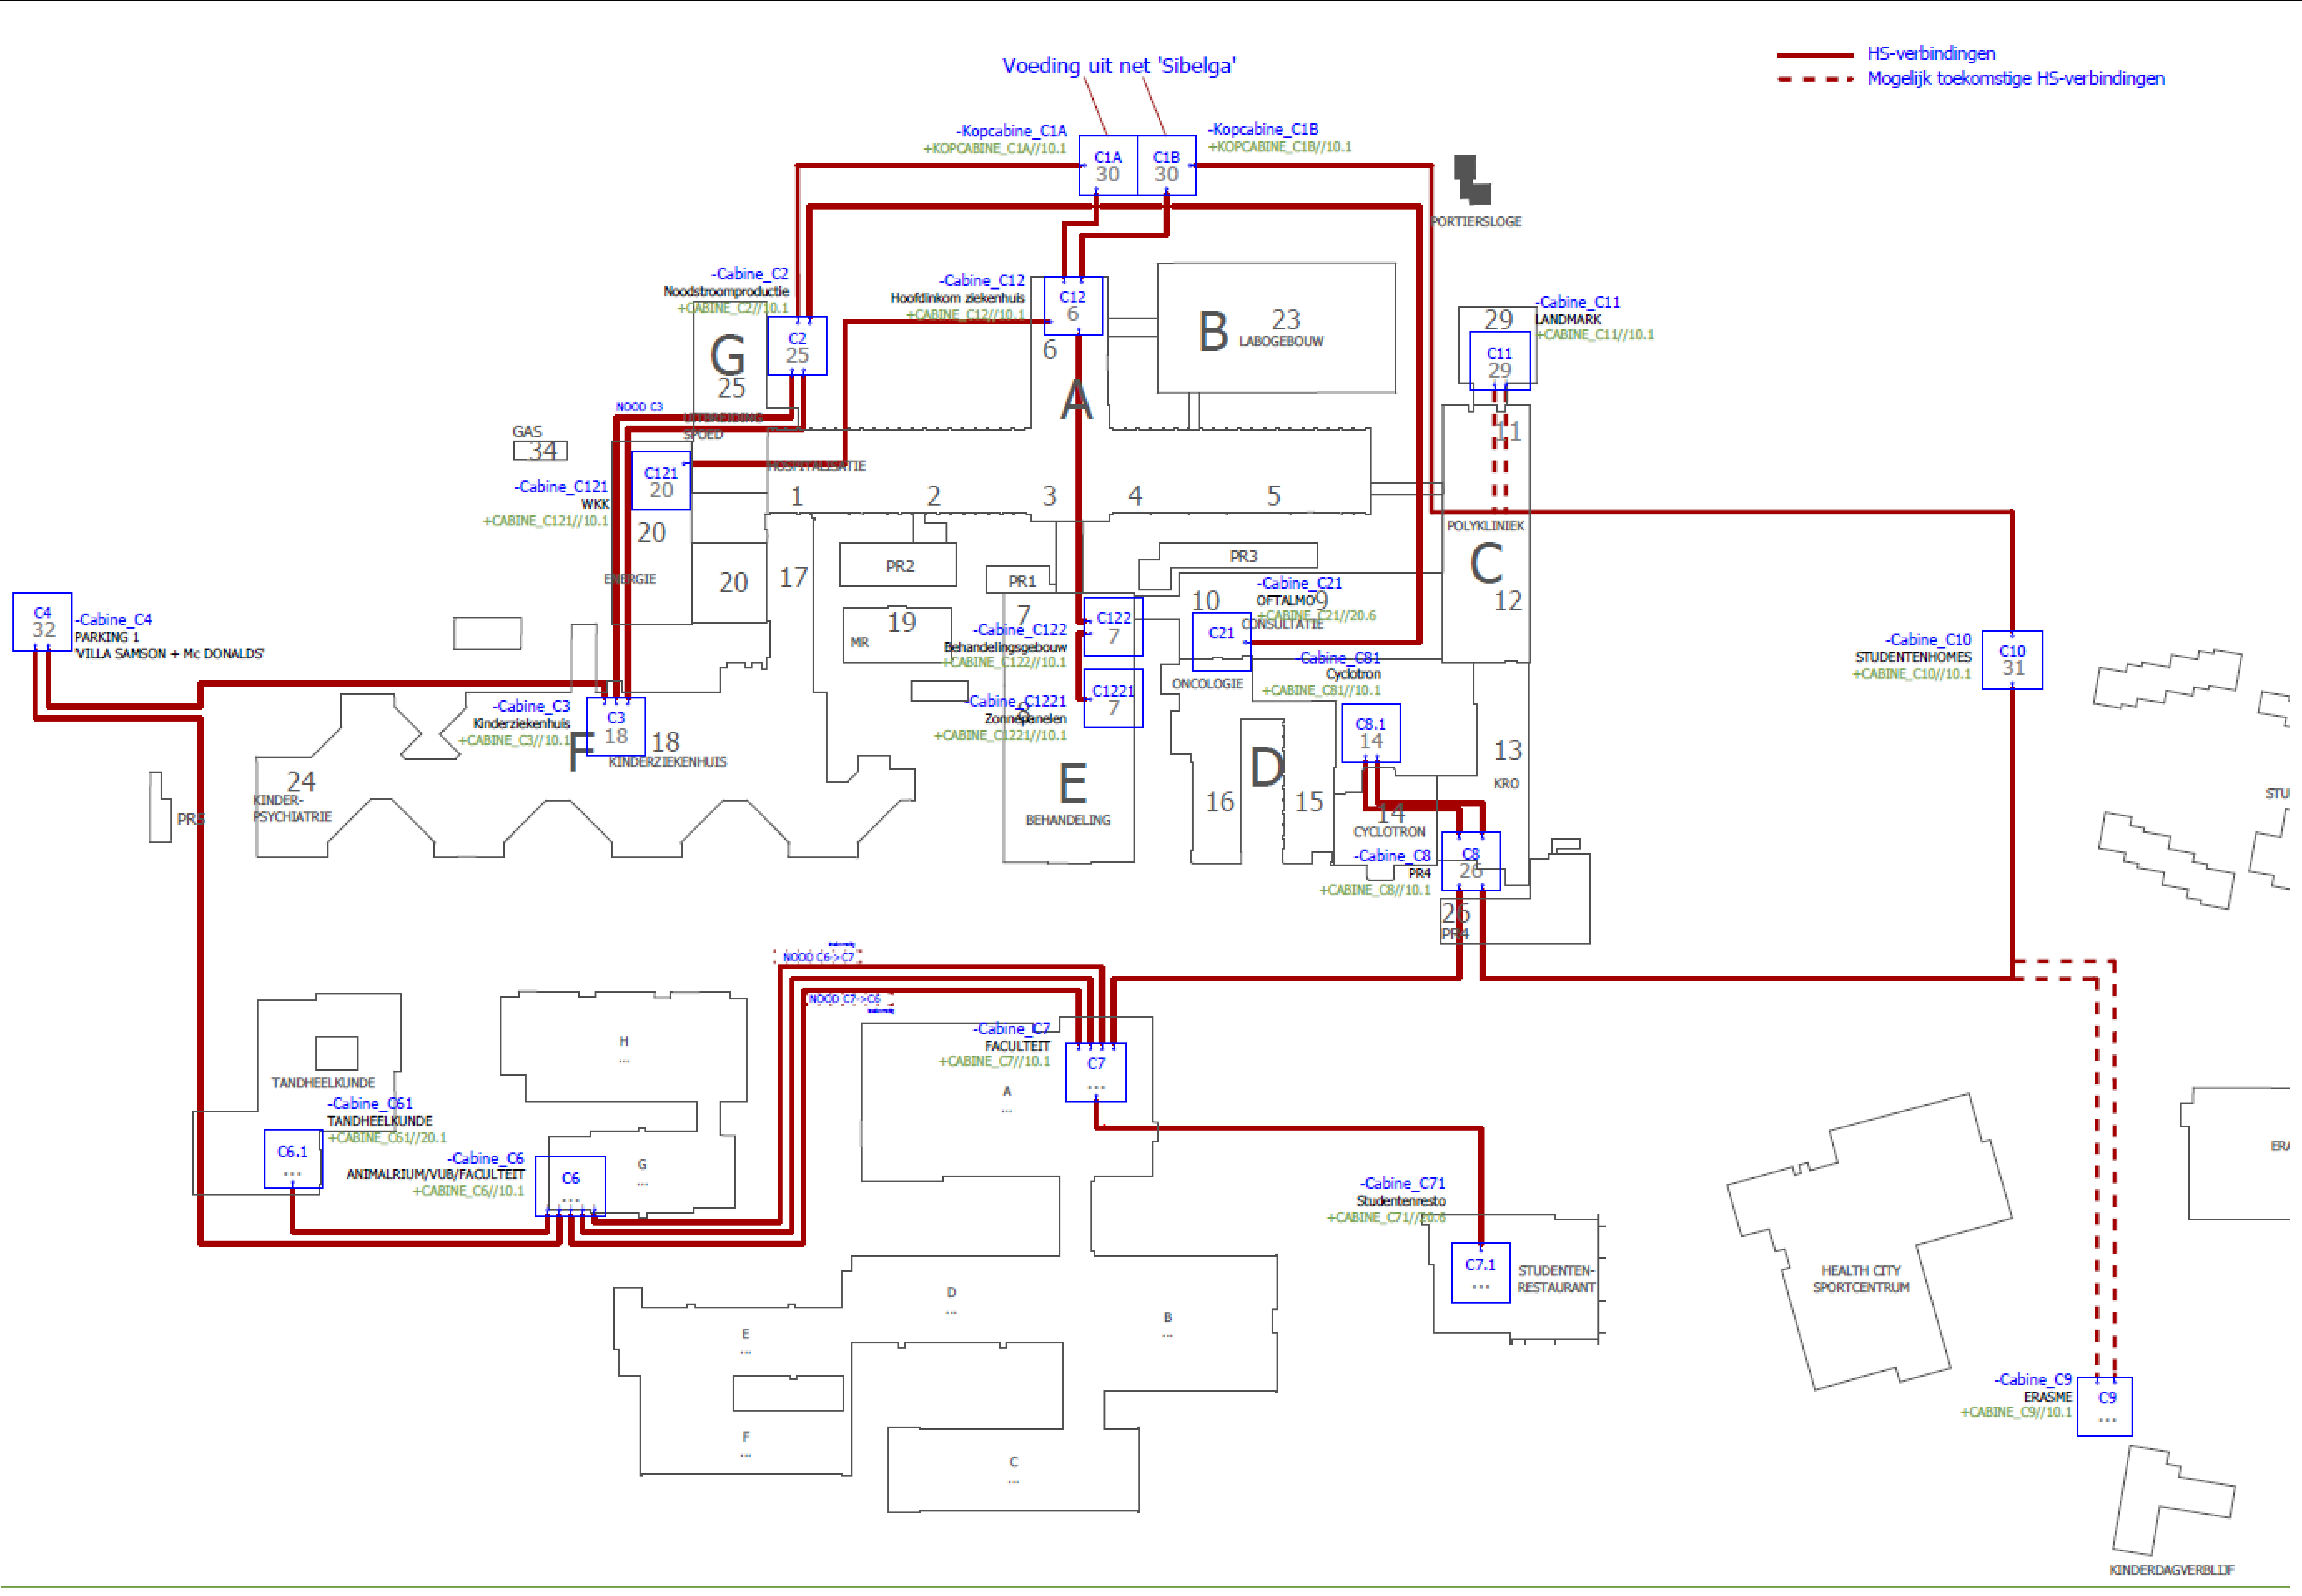
\includegraphics[width=0.78\textwidth]{vub/context/campus_site_layout.pdf}}
        \caption{\acs{UZB} electricity distribution network layout}
        \label{fig:bhc_site_layout}
    \end{figure}
\end{frame}

% \subsection{4 Phases}
\begin{frame}
    \frametitle{4 Phases -- I}
    \vspace*{\fill}
    \begin{columns}[onlytextwidth, c]
        \begin{column}{.47\textwidth}
            \begin{exampleblock}{Data sources}
                \begin{itemize}
                    \item Tries to reflect reality
                    \item Limited dataset
                    \item 15-minute ``electricity'' data
                    \item Also metedata source
                \end{itemize}
                Example:\\
                \texttt{root/NodeC3/Transformer\\
                    0302/ConsumerEnergy/\\
                    Bord\_Radiologie.csv}
            \end{exampleblock}
        \end{column}

        \begin{column}{.52\textwidth}
            \begin{figure}[ht]
                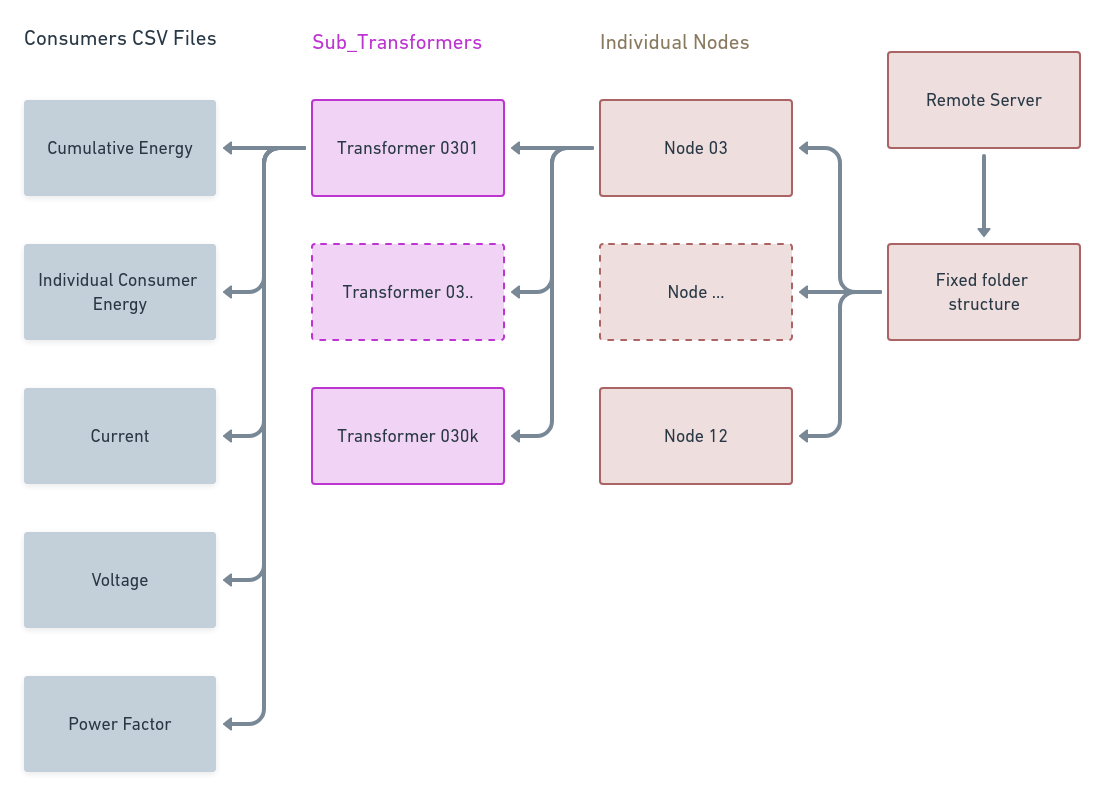
\includegraphics[width=\textwidth]{vub/flowcharts/folder_tree.png}
                \caption{\acs{VUB}'s folder tree structure}
            \end{figure}
        \end{column}
    \end{columns}
    \vspace*{\fill}
\end{frame}

\begin{frame}
    \frametitle{4 Phases -- II \& III}
    \vspace*{\fill}
    \begin{columns}[onlytextwidth, c]
        \begin{column}{.47\textwidth}
            \begin{exampleblock}{Commissioning}
                \begin{itemize}
                    \item \ac{SFTP}
                    \item automate remote access
                    \item automate ingestion
                \end{itemize}
            \end{exampleblock}
        \end{column}
        \begin{column}{.52\textwidth}
            \begin{exampleblock}{Data Management}
                \begin{itemize}
                    \item Multi processing script
                    \item Parsing, cleaning and tagging % w/ Pandas
                    \item Writing DB ``measurement''  %for each node
                \end{itemize}
            \end{exampleblock}
        \end{column}
    \end{columns}
    \begin{figure}[ht]
        \includegraphics[width=\textwidth]{vub/flowcharts/data-management.png}
        \caption{\acs{VUB}'s data ingestion flowchart}
    \end{figure}
    \vspace*{\fill}
\end{frame}

\begin{frame}
    \frametitle{4 Phases -- IV}
    \vspace*{\fill}
    \begin{columns}[onlytextwidth, c]
        \begin{column}{.47\textwidth}
            \begin{exampleblock}{Analysis}
                \begin{itemize}
                    \item Lorem
                    \item Ipsum
                    \item Sed 
                    \item Dolore
                \end{itemize}
            \end{exampleblock}
        \end{column}
        \begin{column}{.52\textwidth}
            \begin{figure}[ht]
                \begin{subfigure}{\textwidth}
                    \centering
                    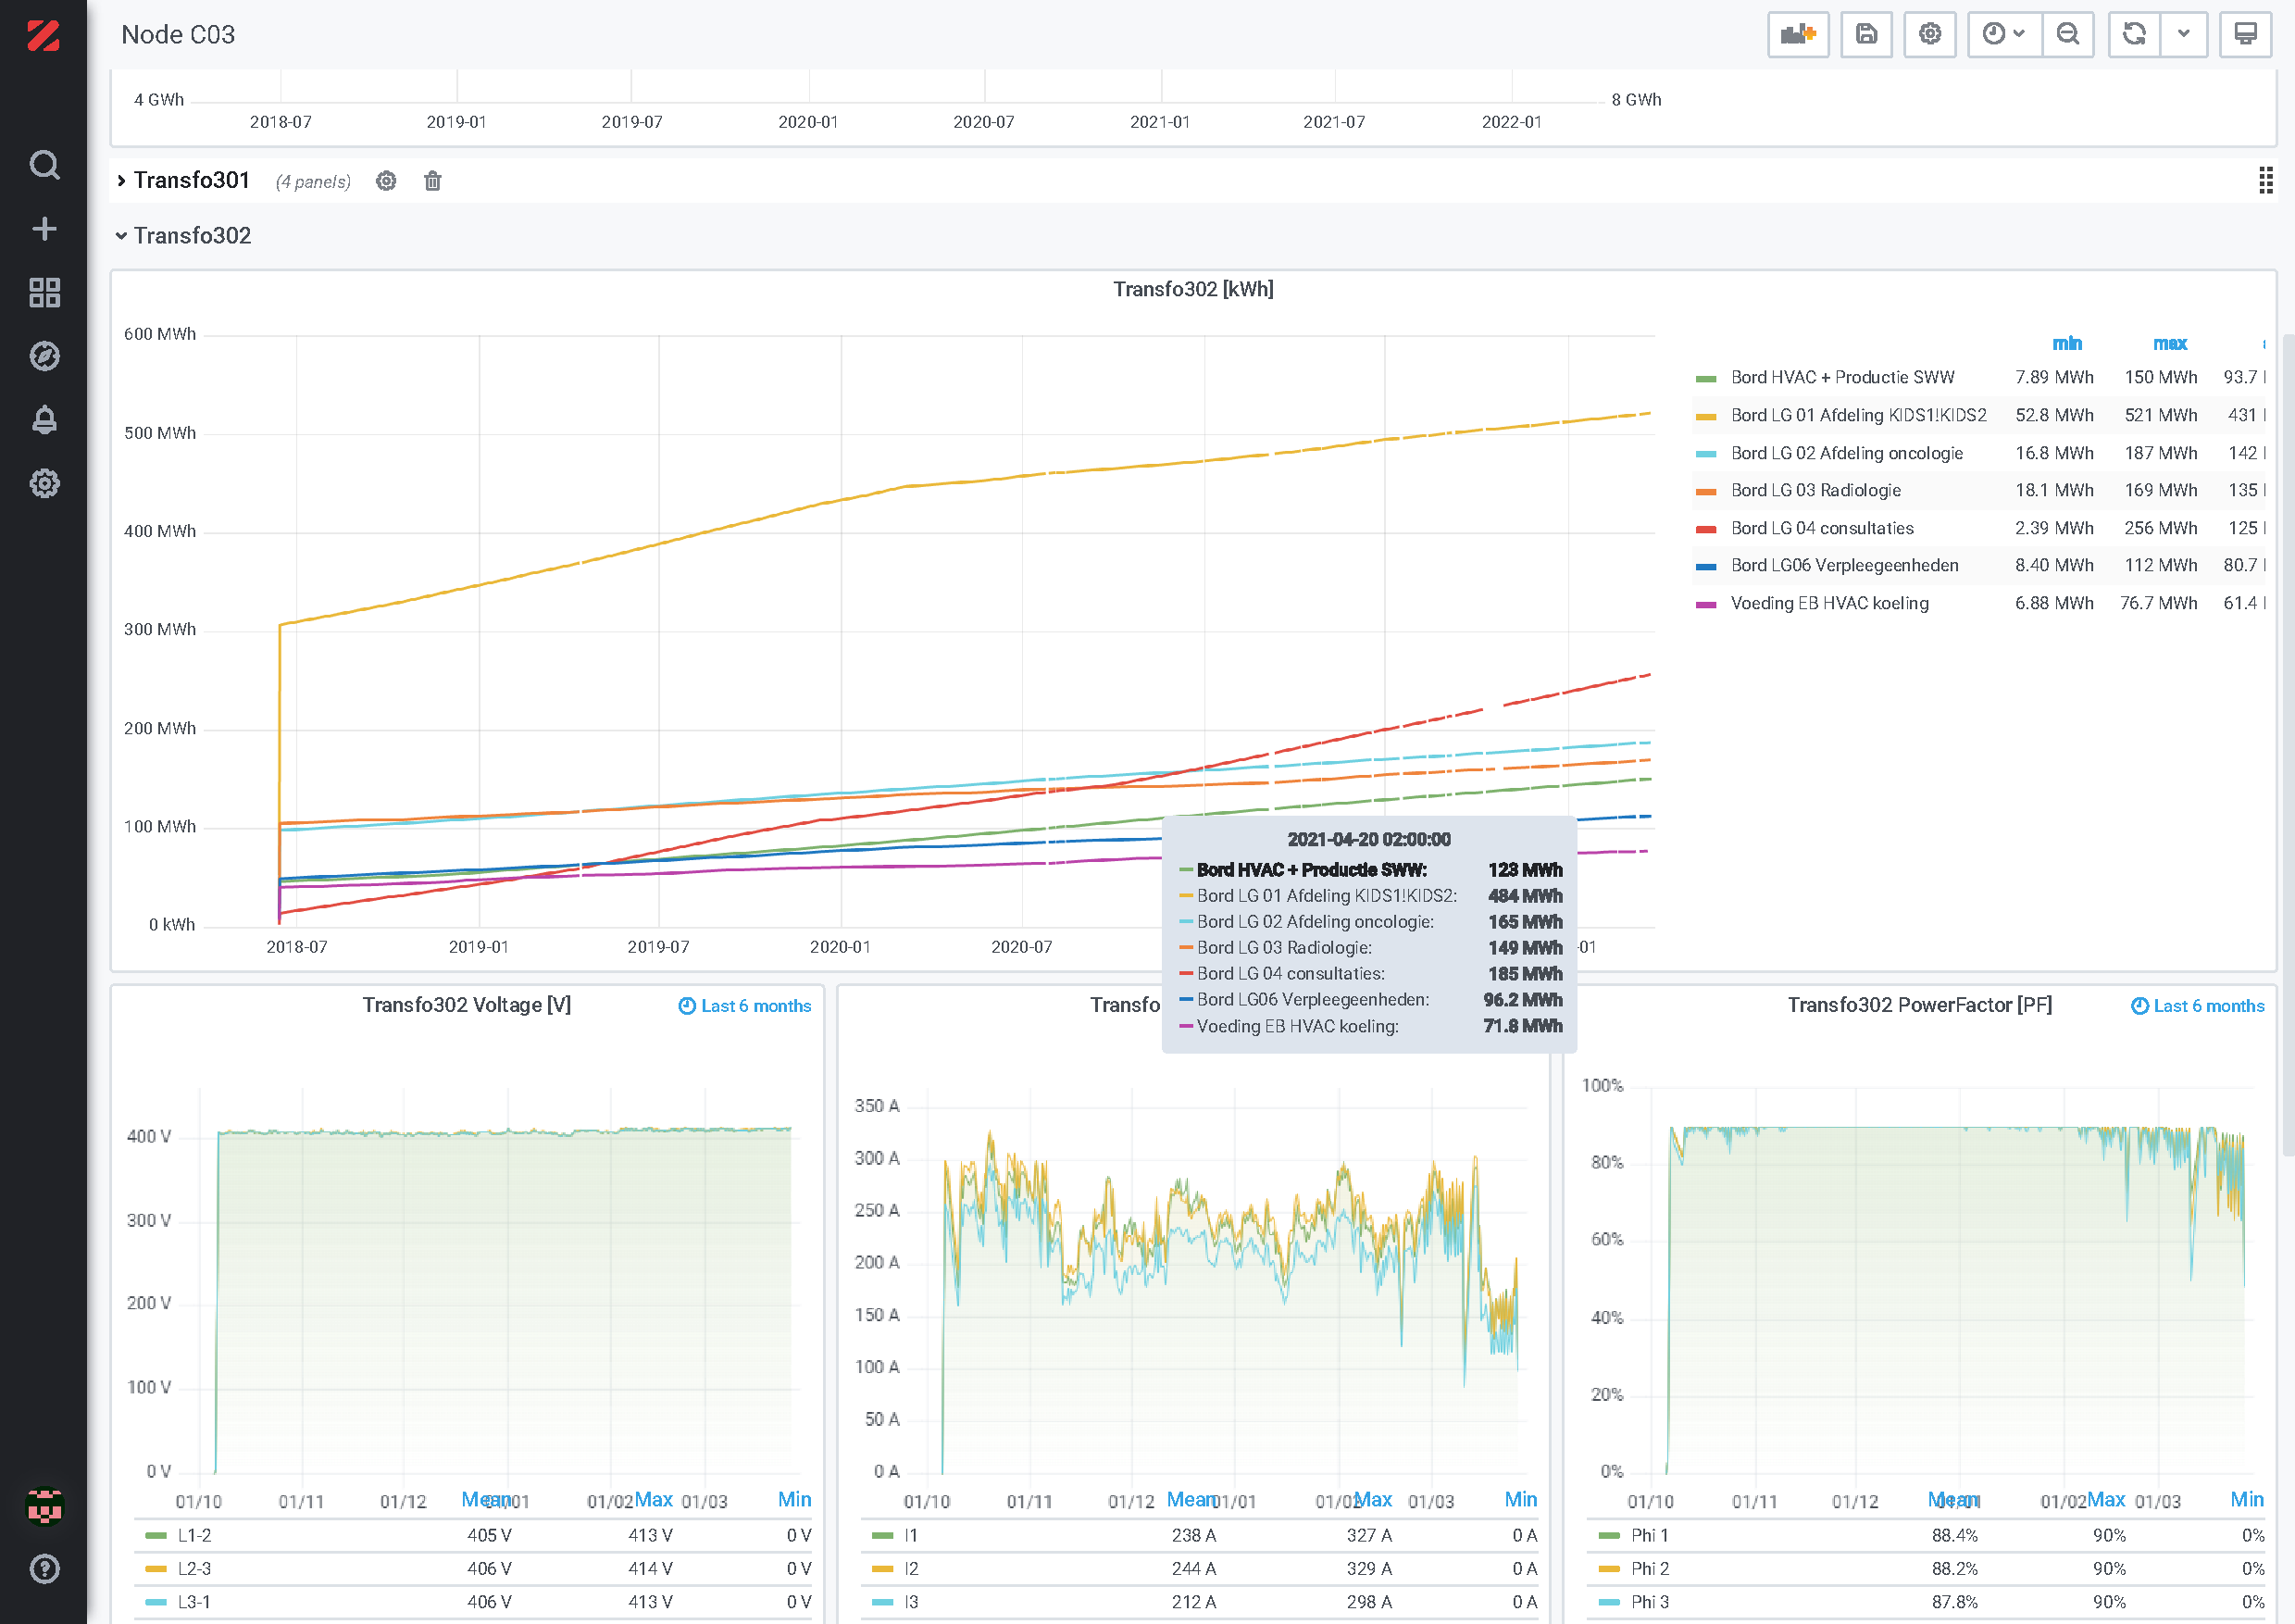
\includegraphics[clip, trim=0 0 0.1cm 3.5cm, width=0.8\textwidth]{vub/grafana/node_c03_transfo302_raw.pdf}
                    \caption{Transformer--302 raw data dashboard}
                \end{subfigure}
                \begin{subfigure}{\textwidth}
                    \centering
                    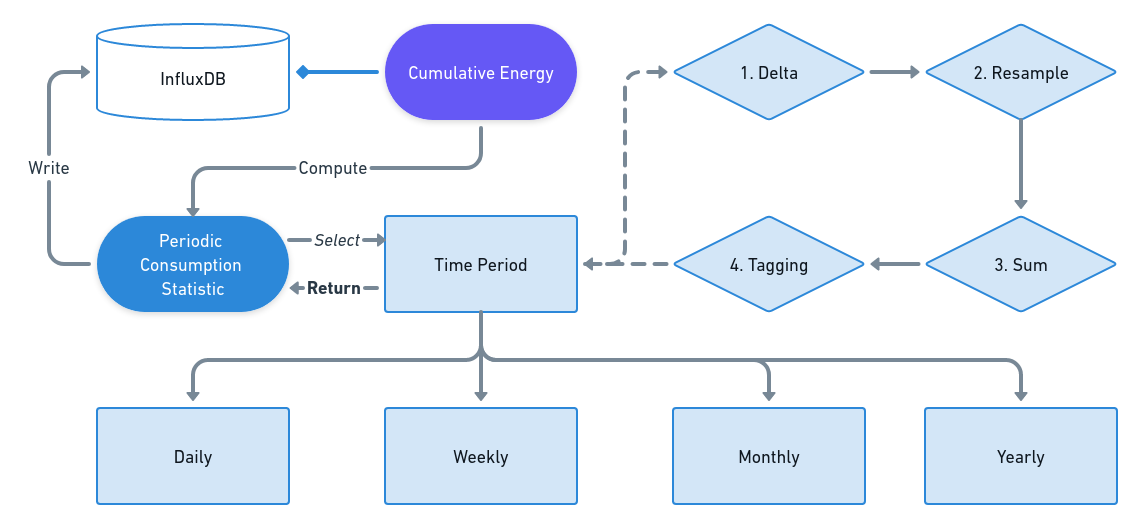
\includegraphics[width=0.8\textwidth]{vub/flowcharts/analystic_flowchart.png}
                    \caption{\acs{VUB}'s analytics chart}
                \end{subfigure}
            \end{figure}
        \end{column}
    \end{columns}
    \vspace*{\fill}
\end{frame}


% \begin{frame}
%     \frametitle{Results}
%     \vspace*{\fill}
%     These plots were then discussed with a more experienced colleague, who had more domain knowledge.
%     He also continued with the analysis.
%     % decided not to discuss his insights, here
%     % in this report, as they are not the result of my work but a more direct consequence.
%     % Slide 2
%     \begin{figure}[htp]
%         \begin{subfigure}{.495\textwidth}
%             \includegraphics[width=1.01\textwidth]{stumabo/analysis/1Hz-ad-hoc.pdf}
%             \caption{1Hz RMS values}
%             \label{fig:stu_1Hz_rms}
%         \end{subfigure}
%         \begin{subfigure}{.495\textwidth}
%             \includegraphics[width=1.01\textwidth]{stumabo/analysis/60Hz-ad-hoc.pdf}
%             \caption{60Hz RMS values}
%             \label{fig:stu_60Hz_rms}
%         \end{subfigure}
%         % \begin{subfigure}{\textwidth}
%         %     \includegraphics[width=\textwidth]{stumabo/analysis/1Hz-vs-60Hz.pdf}
%         %     \caption{\texttt{1Hz} and \texttt{60Hz} RMS values}
%         %     \label{fig:stu_1_vs_60}
%         % \end{subfigure}
%         \caption{RMS amplitude comparison between low and high frequency data}
%         \label{fig:stu_3_rms}
%     \end{figure}

%     \vspace*{\fill}
% \end{frame}


% \begin{frame}
%     \frametitle{Findings}
%     \vspace*{\fill}

%     The \textit{ad-hoc} analysis showed some insightful findings:
%     \begin{enumerate}
%         \item station one, \textcolor{blue}{blue} side, has higher vibration than expected
%         \item station two is the main source of vibration as we hoped it would be
%         \item the cooling fluid, while drying, cause higher vibrations.
%     \end{enumerate}

%     \begin{alertblock}{Counter-intuitive result}
%         Vibration amplitudes ($RMS_{X}$), along the blade going through the grinding stone stations, seemed more
%         prominent than in $Y$ direction, perpendicular to the blade direction.
%     \end{alertblock}

%     The stones turning would intuitively cause
%     more vibrations perpendicular ($Y, Z$) to their rotating axe, not along ($X$).\\
%     After successfully double-checking the whole stack we can confirm that, indeed, $X$ and $Y$ are \structure{not} switched.
%     \vspace*{\fill}
% \end{frame}